% !TEX root = ../main.tex

\section{Sequential Monte Carlo}
\label{sec:part:smc}

\subsection{Non-Markovian State-Space Models}
\label{sec:part:smc:nmssm}

Although SMC can be used for for an arbitrary series of targets as we will explain
in Section INSERT, we will mostly introduce it in the context of non-Markovian state-space
models (NMSSMs).  NMSSMs are probabilistic models over a set of latent variables 
$x_t \in \mathcal{X}_t, \; \forall t = 1:T$
and observed variables $y_t \in \mathcal{Y}_t, \forall t = 1:T$.  
%We can further consider the model to be parameterized by $\theta \in \Theta$ which
%we will for now presume is known.
They are similar to
the HMM introduced in~\ref{sec:bayes:paradigm:graph}, but different by not
making the Markov assumption.  This leads to the graphical model shown in Figure~\ref{fig:part:nmssm}.
They are fully defined by an initial density $\mu (x_1)$,
a series of transition densities $f_{t} (x_t | x_{1:t-1})$, and a series of
emission densities $g_{t} (y_t | x_{1:t})$ as follows
\begin{subequations}
\label{eq:part:ssm}
\begin{align}
x_1 &\sim \mu(x_1), \\
x_t | x_{1:t - 1} &\sim f_{t}(x_t | x_{1:t - 1}), \\
y_t | x_{1:t} &\sim g_{t}(y_t | x_{1:t}).
\end{align}
\end{subequations}
which gives a joint density of
\begin{align}
\label{eq:part:jointdistribution}
p(x_{1:T}, y_{1:T}) = \mu(x_1) \prod_{t = 2}^T f_{t}(x_t | x_{1:t - 1}) \prod_{t = 1}^T g_{t}(y_t | x_{1:t}).
\end{align}
with the standard relationship that this is proportional to the posterior
$p(x_{1:T} | y_{1:T}) \propto p(x_{1:T}, y_{1:T})$.  Note the
key self-similarity relationship: the intermediate posterior of the first $t$ latent variables
given the first $t$ observations is
\begin{align*}
p(x_{1:t} | y_{1:t}) \propto \mu(x_1) \prod_{\tau = 2}^t f_{\tau}(x_{\tau} | x_{1:\tau - 1}) \prod_{\tau = 1}^t g_{\tau}(y_{\tau} | x_{1:\tau}).
\end{align*}

There are two common tasks that one wishes to carry out for this model: \emph{filtering} and
\emph{smoothing}.  Smoothing corresponds to the standard Bayesian inference task where we
want to infer about the latent variables conditioned on all the observations.  In filtering
we care about the posterior given the observations
so far $p(x_t | y_{1:t})$.  Filtering is typically done in tasks such as tracking and signal
processing where the inference is being done online and the main task is forward prediction.
In other words, we do not know all the $y_{1:T}$ upfront but have a series of inference problems
where we wish to predict $y_{t+1},y_{t+2},\dots$ given the observations so far $y_{1:t}$.  Our
focus will be on smoothing, but we note that the this is equivalent to the filtering distribution
at the last step and so most of the ideas directly transfer.

If the model is in fact Markovian with Gaussian or discrete transition distributions and Gaussian
emission distributions, then the solution can be calculated analytically using the \emph{Rauch-Tung-Striebel}
smoother~\citep{rauch1965maximum} and \emph{forward-backward} algorithm~\citep{rabiner1986introduction} respectively.
The former corresponds to the class of Kalman filter~\citep{kalman1960new} and Kalman smoother~\citep{rauch1965maximum}
algorithms.  This are often used a linear Gaussian approximation for Bayesian modeling dynamic of systems and
a are a good example of where approximations are often made in Bayesian approaches in the interest of
tractability.  SMC will allow us to perform inference in similar models, amongst many others, without requiring
such assumptions to be made.  Naturally this will come at the cost of having access to a closed-form solution.

\begin{figure}[t]
	\centering 
	% !TEX root = ../main.tex

\begin{tikzpicture}

\node[latent, minimum size=27pt] (x1) {$x_1$};
\node[latent, right=1.4cm of x1, minimum size=27pt] (x2) {$x_2$};
\node[right=1.4cm of x2] (x3) {{\tiny $\bullet \; \bullet \; \bullet$}};
\node[latent, right=1.4cm of x3, minimum size=27pt] (x4) {$x_{T\text{-}1}$};
\node[latent, right=1.4cm of x4, minimum size=27pt] (xT) {$x_T$};

\node[obs, below=of x1, minimum size=27pt] (y1) {$y_1$};
\node[obs, below=of x2, minimum size=27pt] (y2) {$y_2$};
%\node[obs, below=of x3] (y3) {$y_3$};
\node[obs, below=of x4, minimum size=27pt] (y4) {$y_{T\text{-}1}$};
\node[obs, below=of xT, minimum size=27pt] (yT) {$y_T$};

%\node[latent, above=of x1, xshift=-1.2cm, minimum size=27pt] (t) {$\theta$};

\edge {x1} {x2,y1} ; %
\edge {x2} {x3,y2} ; %
\edge {x3} {x4} ; %
\edge {x4} {xT,y4} ; %
\edge {xT} {yT} ; %

%\edge {t} {x1,x2};
%\edge[bend left=0] {t} {x4};
%\edge[bend left=10] {t} {xT};

\edge[bend left=30] {x1} {x4}
\edge[bend left=35] {x1} {xT}
\edge[bend left=20] {x2} {xT}

\edge[bend left=0] {x1} {y2,y4,yT}
\edge[bend left=10] {x2} {y4,yT}
\edge[bend left=0] {x4} {yT}

\end{tikzpicture}
	\caption{DAG for a non-Markovian state space model.  Note there are all also multiple dependencies
		for the nodes summarized in the dots.
		\label{fig:part:nmssm}}
\end{figure}

\subsection{Sequential Importance Sampling}
\label{sec:part:smc:sis}

\begin{algorithm}[tb]
	\caption{Sequential Importance Sampling}
	\label{alg:part:sis}
	\begin{spacing}{1.2}
		\begin{algorithmic}[1]
			\renewcommand{\algorithmicrequire}{\textbf{Inputs:}}
			\renewcommand{\algorithmicensure}{\textbf{Outputs:}}			 
			\Require model $p(x_{1:T},y_{1:T})$, data $y_{1:T}$, proposals $q_1,\dots,q_T$, number of samples $N$
			\For{i=1,\dots,N}	
			\State $x_1^i \sim q_1(x_1)$
			\State $w_1^i = \frac{g_1(y_1|x_1^i) \mu(x_1^i)}{q_1(x_1^i)}$
			\For{$t = 2$ {\bfseries to} $T$}
			\State $x_t^i \sim q_t(x_t | x_{1:t-1}^i)$ 
			\State Set $x_{1:t}^i = (x_{1:t-1}^{i},x_t^i)$
			\State $w_t^i = w_{t-1}^i \frac{g_t(y_t|x_{1:t}^i) f_t(x_t^i | x_{1:t-1}^{i})}{q_t(x_t^i|x_{1:t-1}^{i})}$
			\EndFor
			\EndFor
			\Ensure weighted samples $\left\{x_{1:T}^i,w_T^i\right\}_{i=1}^N$
		\end{algorithmic}
	\end{spacing}
\end{algorithm}


In Section~\ref{sec:inf:foundation:importance:unk-f} we showed that importance sampling weights
are multiplicative (see~\eqref{eq:inf:prod-imp-weights}) and thus to sample from a joint
distribution, one can first importance sample from a marginal distribution and then importance
sample from the respective conditional distribution, with the sample weight corresponding to the
product of the two individual weights.  More generally, one can carry out \emph{sequential importance
	sampling} (SIS) where we sample from a series of target distributions $(\pi_t(x_{1:t}))_{t = 1}^T$ of 
increasing spaces $(\mathcal{X}_1 \times \dots \times \mathcal{X}_t)_{t = 1}^T$ by first making
an importance sampling approximation for $\pi(x_1)$ and sequentially update our approximation from
$\pi_t(x_{1:t})$ to $\pi_{t+1}(x_{1:t+1})$ by doing importance sampling updates and taking the product of
the weights.  This is easiest to see in the NMSSM case were we will first approximate $p(x_1 | y_1)$
using importance sampling and then importance sample each 
\[
p (x_t | x_{1:t-1}, y_{1:t})=p(x_t | x_{1:t-1}, y_t)\propto f_{t}(x_t | x_{1:t-1}) g_{t}(y_t | x_{1:t})
\]
noting that $x_t$ is independent of $y_{1:t-1}$ given $x_{1:t-1}$.  Presuming a set of proposals 
$q_1(x_1), q_t(x_t | x_{1:t-1})$, we will calculate importance weights as follows
\begin{subequations}
	\label{eq:part:sis-weights}
\begin{align}
w_1 (x_1) &= \frac{\mu (x_1)g_{t}(y_1 | x_1)}{q_1(x_1)} \\
w_t (x_{1:t}) &= w_{t-1} (x_{1:t-1}) \frac{g_{t}(y_t|x_{1:t}) f_{t}(x_t | x_{1:t-1})}{q_t(x_t|x_{1:t-1})}.
\end{align}
\end{subequations}
Once completed this will produce a weighted sample $\{\hat{x}_{1:T},w_T(\hat{x}_{1:T})\}$ for 
$p(x_{1:T} | y_{1:T})$.  A summary of the SIS process is given in Algorithm~\ref{alg:part:sis}.

Because SIS produces are pure importance sampling estimate, it will share all the desirable properties
of importance sampling introduced in Section~\ref{sec:inf:foundation:importance}.  In fact, it is just
a particular case of importance sampling because could have produced the same samples and weights
by sampling $x_{1:T} \sim q_1(x_1) \prod_{t=2}^{T} q_t (x_t | x_{1:t-1})$ and then calculating the
corresponding importance weight $w_T(x_{1:T})$ in one go. As such, 
SIS is not on its own very useful.  Its utility will be when it is combined with resampling as we describe next.

\subsection{SMC for Non-Markovian State Space Models}
\label{sec:part:smc:smc-nmssm}

Sequential Monte Carlo (SMC)~\citep{gordon1993novel,doucet2001sequential,doucet2009tutorial} , or particle filtering 
as it is sometimes known,\footnote{We avoid the name
	particle filtering as it often implies that one is only interested in the filtering distribution, whereas
	most of the tasks we are interested in will target the smoothing distribution.} 
is a powerful and general purpose inference algorithm that has been successfully
applied to a wide range of fields such as signal processing~\citep{candy2016bayesian}, econometrics~\citep{creal2012survey}, 
and probabilistic programming~\citep{wood2014new}.  SMC builds on SIS by interleaving the sampling
with resampling steps, the latter
of which was introduced in Section~\ref{sec:inf:foundation:resampling}.
The key idea is to exploit the structure of a model by breaking down the overall 
inference problem into a series of target distributions which get incrementally closer to the 
distribution of interest.  Transitioning from one intermediary distribution to the next typically
forms a far simpler inference problem that directly approximating the original target.  The critical difference
to SIS is that
the information gained from approximating these intermediary distributions can be exploited,
reallocating resources to areas likely to have high posterior mass in the final target distribution
through the resampling process.  The simplest, but most common form of SMC, which simply interleaves
\emph{propagating} samples from one target to the next and resampling the particle system, is sometimes known
as \emph{sequential importance resampling} and will be our main focus.
A characterization of the method is shown in Figure~\ref{fig:part:smc_explan}.  

\begin{figure}[t]
	\centering 
	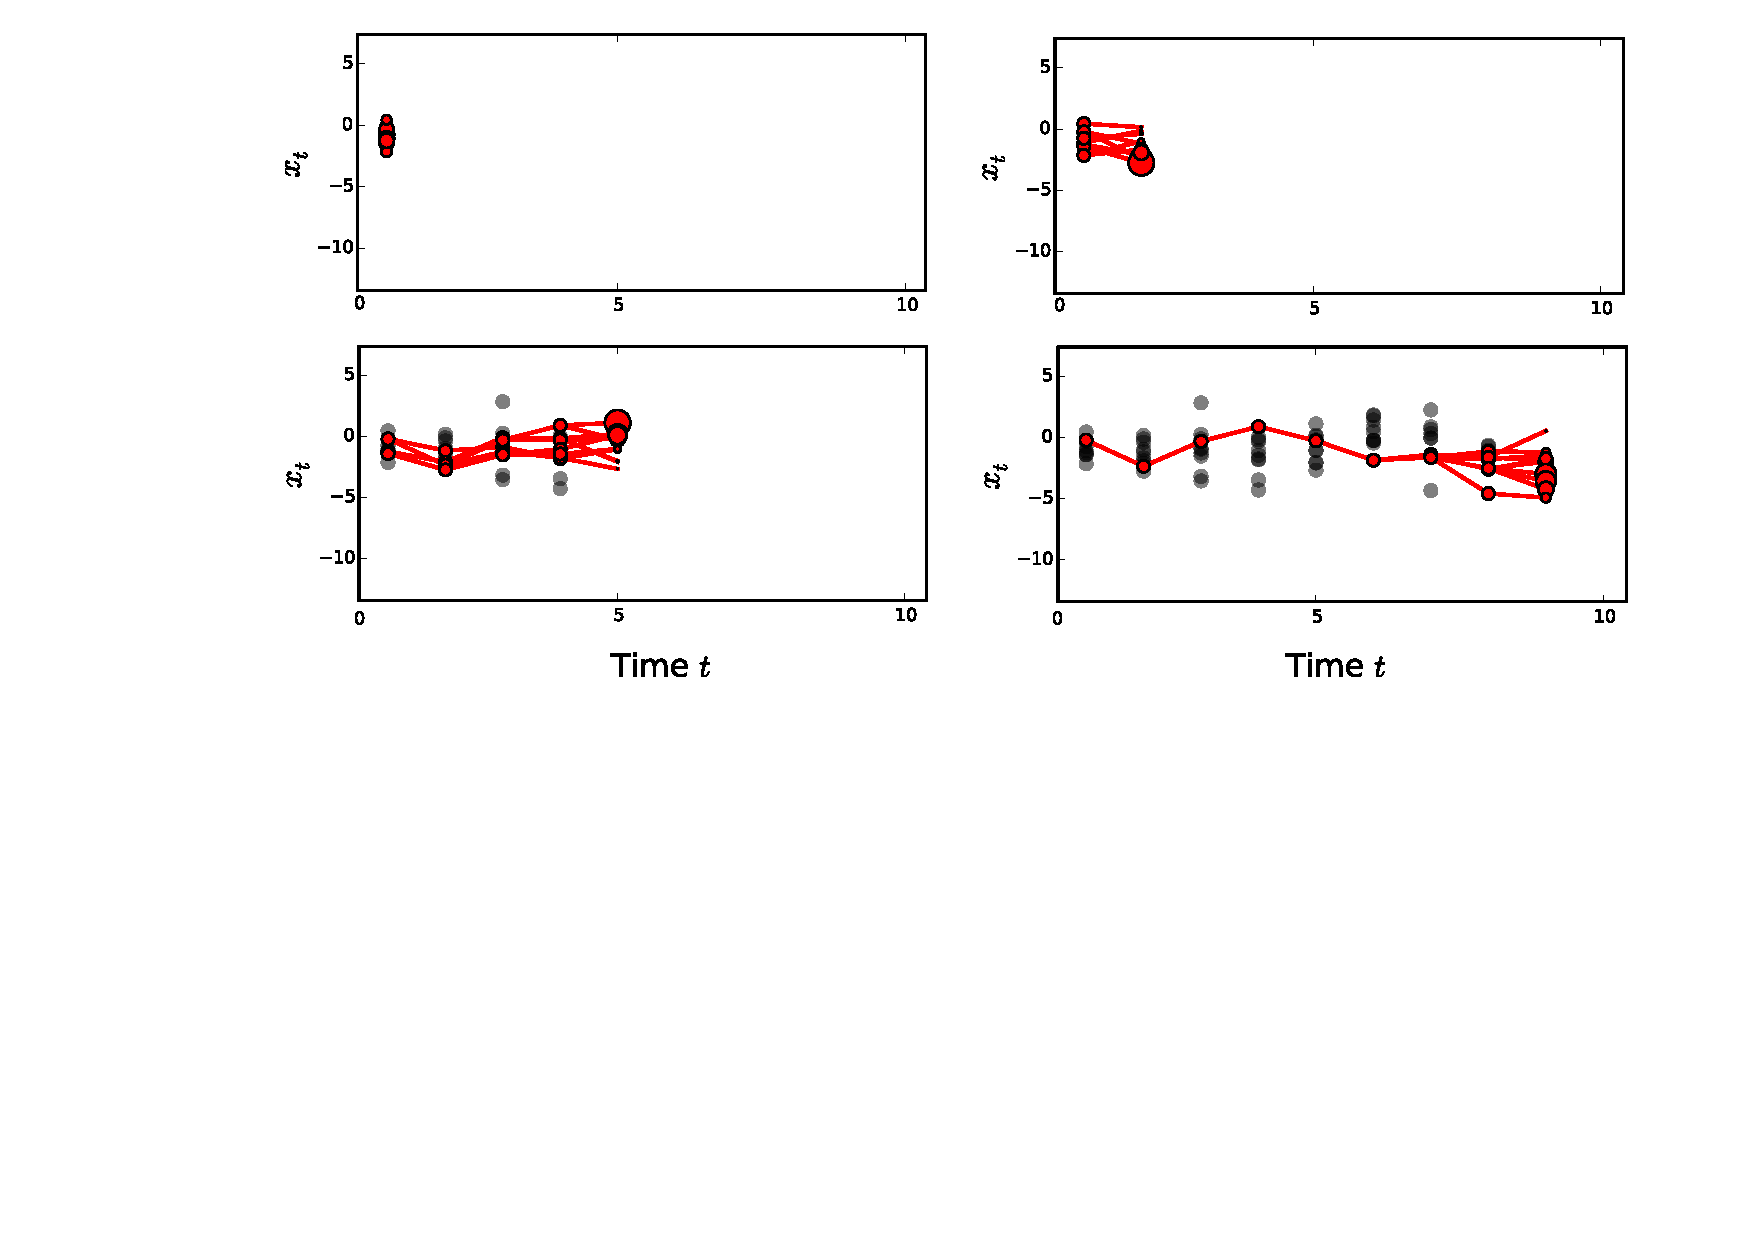
\includegraphics[width=\textwidth]{part/figures/smc_explan}
	\caption{Characterization of the SMC method for a non-Markovian state space model.  At the first time step (top left) 
		we perform importance sampling to approximate $p(x_1 | y_1)$ in the normal way, given a particle system, or population
		of weighted samples $\{x_1^i,w_1^i\}_{i=1}^N$.  Here each sample is shown by a red blob whose size reflects the weight
		of the particle.  The set of particles are then resampled to produce an unweighted set of particles approximating
		$p(x_1 | y_1)$.  For each of these samples, importance sampling is then used again to produce samples for $x_2$
		by sampling from $q_2 (x_2 | x_1)$ and applying a new importance weight (top right).  Note that, unlike for SIS,
		the importance weights are not propagated from one time step to the next (see Algorithm~\ref{alg:part:smc}).
		We now again have a weight particle set $\{x_{1:2}^i,w_2^i\}_{i=1}^N$, for which we again perform a resampling
		step to produce an unweighted set of particles.  The process continues in the same way, eventually return in the
		final set of samples $\{x_{1:T}^i,w_T^i\}_{i=1}^N$.  Note that over time, many of the generated samples are
		discarded by the system (shown in gray) during the resampling step.  Here we see (bottom left) then after
		many time steps, then our particle set become \emph{degenerate}.  Here we have multiple distinct samples for $x_9$, but
		all our samples share the same \emph{ancestors} for $t=1:6$, i.e. each $x_t^i$ in our final sample set is
		the same for $t\le6$.  We will return to discuss this in Section INSERT.
		\label{fig:part:smc_explan}}
\end{figure}

To see the intuition of why resampling provides the desired resource reallocation, consider what happens 
to the relative weights of different particles in a population are propagated through the SIS algorithm at the
same time.  It is easy to see that these weights will quickly diverge, typically exponentially quickly in the
number of time steps (see Section~\ref{sec:inf:foundation:curse}), and our effective sample size 
(see Section~\ref{sec:inf:foundation:ess}) will rapidly diminish.  It is now rather pointless to continue to
propagate the samples with negligible weight through the system as the chance these will have a significant
weight by the end of sampling is very low.  We therefore desire a principled way of ``killing off'' these
low weight particles and replacing them with higher weight ones.  As we showed in Section~\ref{sec:inf:foundation:resampling},
resampling gives us a method for generating unweighted samples from a population of weighted samples.
We explained that if these samples are just going to be used directly for estimation then this is strictly
detrimental procedure.  However, if we are going to use the samples as a starting point for further sampling this
will no longer apply.  This is because though resampling itself only duplicates existing particles, rather
than producing new ones, if the duplicate samples are extended independently at the next iteration, they will
produce distinct (albeit heavily correlated) samples at the next iteration.  In other words if we have two samples
$x_{1:t}^1$ and $x_{1:t}^2$ such that $w_t^2/w_t^1 \approx 0$ then it is more beneficial for us to generate both
samples at the next stage using $x_{t+1}^i \sim p(x_{t+1} | x_{1:t}^1, y_{1:t})$ for $i=1,2$ than to use
$x_{1:t}^2$ to sample $x_{t+1}^1$.  This will not improve our representation of $x_{1:t}$, but it will, in
general, give a better representation of the marginal distribution of $x_{t+1}$ and the joint distribution
$x_{1:t+1}$.   Note that any of the resampling schemes introduced in Section~\ref{sec:inf:foundation:resampling}
will give rise to valid SMC schemes.

To introduce the \smc method more formally, we consider approximating a sequence of target distributions: in our NMSSM
 case $p(x_{1:t}|y_{1:t}) = p(y_{1:t})^{-1} p(x_{1:t},y_{1:t}), ~t=1,\ldots,T$. 
At each time step $t$ we 
%assume we have access to 
generate a \emph{particle system}
$\{(x_{1:t}^i,w_{t}^i)\}_{i=1}^N$ which provides a weighted approximation  to $p(x_{1:t}|y_{1:t})$. Given such a weighted particle system at time $t-1$, this 
%The particle system is then
is propagated forward in time to $t$ by first drawing an ancestor variable $a_{t-1}^i$ for each particle from its corresponding distribution:
\begin{align}
\label{eq:part:anc-sample}
\Prb(a_{t-1}^i = \ell) &= \nw_{t-1}^\ell.
&
\ell&=1,\ldots,N,
\end{align}
where $\nw_{t-1}^\ell = w_{t-1}^\ell / \sum_i w_{t-1}^i$. This is equivalent to our process of resampling, but
will provide poor precise notation when we come to deal with PMCMC methods in Section~\ref{sec:part:pmcmc}
where we see that it is beneficial to consider our approach as working on an \emph{extended target} comprising
of both the samples for the latent variables and the ancestor variables.  Note that any of the resampling 
methods introduced in Section~\ref{sec:inf:foundation:resampling} can be used for~\eqref{eq:part:anc-sample}.  As
our results their showed that systematic resampling gives the best performance, this should also be used
as the go-to resampling scheme for SMC.

\begin{algorithm}[tb]
	\caption{Sequential Monte Carlo \hfill {\small (all for $i=1,\ldots,N$)}}
	\label{alg:part:smc}
	\begin{spacing}{1.2}
		\begin{algorithmic}[1]
			\renewcommand{\algorithmicrequire}{\textbf{Inputs:}}
			\renewcommand{\algorithmicensure}{\textbf{Outputs:}}				 
			\Require  data $y_{1:T}$, number of particles $N$, proposals $q_t$
			\State $x_1^i \sim q_1(x_1)$
			\State $w_1^i = \frac{g_1(y_1|x_1^i) \mu(x_1^i)}{q_1(x_1^i)}$
			\For{$t = 2$ {\bfseries to} $T$}
			\State $a_{t-1}^i \sim \Discrete\left(\left\{\nw_{t-1}^{\ell}\right\}_{\ell=1}^N\right)$% \tom{We can maybe more general that categorical here?}
			\State $x_t^i \sim q_t(x_t | x_{1:t-1}^{a_{t-1}^i})$ 
			\State Set $x_{1:t}^i = (x_{1:t-1}^{a_{t-1}^i},x_t^i)$
			\State $w_t^i = \frac{g_t(y_t|x_{1:t}^i) f_t(x_t^i | x_{1:t-1}^{a_{t-1}^i})}{q_t(x_t^i|x_{1:t-1}^{a_{t-1}^i})}$
			\EndFor
		\end{algorithmic}
	\end{spacing}
\end{algorithm}

We continue by simulating from some given proposal density $x_t^i \sim q_t(x_t | x_{1:t-1}^{a_{t-1}^i})$ and 
re-weight the system of particles as follows:
\begin{align}
\label{eq:smcweights}
w_t^i = \frac{g_t(y_t|x_{1:t}^i) f_t(x_t^i | x_{1:t-1}^{a_{t-1}^i})}{q_t(x_t^i|x_{1:t-1}^{a_{t-1}^i})},
\end{align}
where $x_{1:t}^i = (x_{1:t-1}^{a_{t-1}^i},x_t^i)$. This results in a new particle system $\{(x_{1:t}^i,w_t^i)\}_{i=1}^N$ that approximates $p(x_{1:t}|y_{1:t})$. This process if detailed in Algorithm~\ref{alg:part:smc}.  Note that after resampling,
all the particles have the same weight and therefore, unlike for SIS, the weights at the previous step
do not feature in the weights at the current time step.

Many intuitions from importance sampling transfer over to SMC.  For example, we can construct our posterior
estimate and calculate expectations in the same way, while we can also use the effective sample size as
a metric of performance.  One of the most importance features that (roughly) translates is that SMC produces the
unbiased estimate for the marginal likelihood 
\begin{align}
\label{eq:part:ML}
\hat Z = \prod_{t=1}^T \frac{1}{N} \sum_{i=1}^N w_{t}^{i}.
\end{align}
as first shown by~\cite{del2004feynman}.  Although this original
proof requires advanced techniques we will not touch on here, we will later show that this results can also be shown
as a consequence of the derivation of PMCMC methods in Section~\ref{sec:part:pmcmc}.  Producing unbiased
estimates of the marginal likelihood has numerous significant advantages.  Firstly, it means that one can combine
results from difference SMC runs and still have an unbiased and consistent estimator for the target.  
The importance of this is that the number of particles $N$, is typically restricted by the availability of memory
and we often want to run more than one \emph{SMC sweep} (i.e. a single run of SMC).
To combine our estimates,
simply weight each sample by the marginal likelihood of its sweep times
its local weight $w_T^i$.  The ability to do this is known as \emph{proper weighting} and we can justify it by
thinking in terms of using a proposal that first samples a full particle set, giving importance weight $\hat Z$, and then sampling a particle
from this set, giving importance weight $w_T^i$.  Our product of these separate weights gives the weight of
the samples.  Nonetheless, one sometimes actually wishes to combine the weights from different SMC sweeps
without including the weight from marginal likelihood weightings.  This is know in the literature as using
islands CITE SOMETHING and it produces biased, but typically lower variance, estimates for the posterior.
Secondly, it means that we can \emph{nest} SMC within other methods as a unbiased estimate of the likelihood.
Such methods are known as pseudo-marginal methods and we will discuss them further in Chapter~\ref{chp:nest}.
This will also be the basis for many PMCMC methods as shown in the next section.

The sequential nature of SMC and the resampling step are crucial in making SMC scalable to large $T$.
The former makes it easier to design efficient proposal distributions as each step need only target 
the next set of variables $x_t \in \mathcal{X}_t$. 
The resampling step then allows the algorithm to focus on promising particles in light of new 
observations, avoiding the exponential divergence between the weights of different samples that 
occurs for importance sampling as $T$ increases.
This can be demonstrated both empirically and theoretically \citep[Chapter 9]{del2004feynman}.
We refer the reader to the review by \citet{doucet2009tutorial} for a more in-depth treatment of SMC.

\subsection{Adaptive Resampling}
\label{sec:part:smc:adapt-resam}

\todo[inline]{Write me}

\subsection{Sequential Monte Carlo for an Arbitrary Series of Targets}
\label{sec:part:smc:arb}

In its most general form, we can consider SMC as targeting an arbitrary
series of unnormalized target distributions $\left\{\gamma_t\right\}_{t=1:T}$ each defined on a space
$\mathcal{X}_t$ with strictly increasing dimension\footnote{This restriction
	can be avoided by using the SMC samplers approach of \citet{del2006sequential}.}
$\mathrm{dim}(\mathcal{X}_{t-1})<\mathrm{dim}(\mathcal{X}_{t})$. 
Let
\begin{align}
\label{eq:part:norm-targets}
\pi_t(x_{1:t}) := \frac{\gamma_t(x_{1:t})}{Z_t}
\end{align}
be the series of normalized targets densities approximated by our SMC scheme
where $\gamma_t(x_{1:t})$ and $Z_t := \int \pi_t(x_{1:t}) dx_{1:t}$
are the corresponding unnormalized targets and normalization constants respectively.
The overall normalization constant for the SMC is given by $Z:=Z_T$.  
Let $q_1(x_1)$ denote the first proposal density and $q_t(x_t | x_{1:t - 1})$ 
the intermediate proposal densities.  The particle weights (assuming resampling is
carried out at each step $t$) are now given by
\begin{align}
w_1^k &= \frac{\gamma_1(x_1^k)}{q_1(x_1^k)} \\
w_t^k &= \frac{\gamma_t({x}_{1:t}^k)}{\gamma_{t - 1}({x}_{1:t - 1}^{a_{t - 1}^k}) q_t(x_t^i|x_{1:t-1}^{a_{t-1}^i})}.
\end{align}
Everything else is then kept as for the NMSSM case.

An upshot of this ability is that we can use SMC in lots of scenarios that do not
actually permit an appropriate breakdown of the target distribution but where we 
can provide guiding distributions to that which we care about.  For example, in a probabilistic
context free grammar we might have a sequential generative model that can be evaluated on the
full dataset at any point.  For example, in~\cite{janz2016probstruct}, we considered the example of doing inference
on the structure and parameters of a GP kernel.  Here we can think of expanding our kernel at each
iteration and our targets as being the posterior on kernel structure and hyperparameters for the GP
for sequentially more complex kernels.\footnote{Technically in this work actually uses a population
	Monte Carlo~\cite{cappe2004population} we uses a series of static targets.  However, we could
	have done this in the same way using only SMC.}  Another example is provided by~\cite{lakshminarayanan2013top}
who use SMC for Bayesian learning of decision trees.  For both these problems, SMC has been used
to exploit the fact that the overall problem can be broken down into a series of increasingly difficult
problems, namely those with an increasingly large prior.